\subsection{Aprendizado de Máquina}

Segundo \space\citeonline{directions_ia_ml_dp}, aprendizado de máquina é uma subcategoria de inteligência artificial que se refere  a detecção de padrões importantes de uma base de dados. As ferramentas utilizadas aumentam a eficiência dos algoritmos para lidar com bases de dados grandes.

Portanto, essa técnica permite ao computador melhorar os resultados com base na experiência, isso indica uma relação direta entre o quanto o programa consumiu de dados e qualidade da solução do problema \space\cite{ml_explicado}. 

Dentro desse nicho existem outros como: redes neurais, algoritmos evolucionários, algoritmos de busca, aprendizado por reforço, dentre outros. \space\cite{ml_oil_gas_industry}.

É possível observar uma hierarquia entre aprendizado de máquina e os principais termos, sendo eles: redes neurais artificiais e aprendizado profundo, ilustrado na \cref{fig:diagrama_ann} \space\cite{ml_and_dp}.

\begin{figure}[ht]
	\caption{Ilustração da relação entre os principais tópicos de aprendizado de máquina}
	\centering % para centralizarmos a figura
	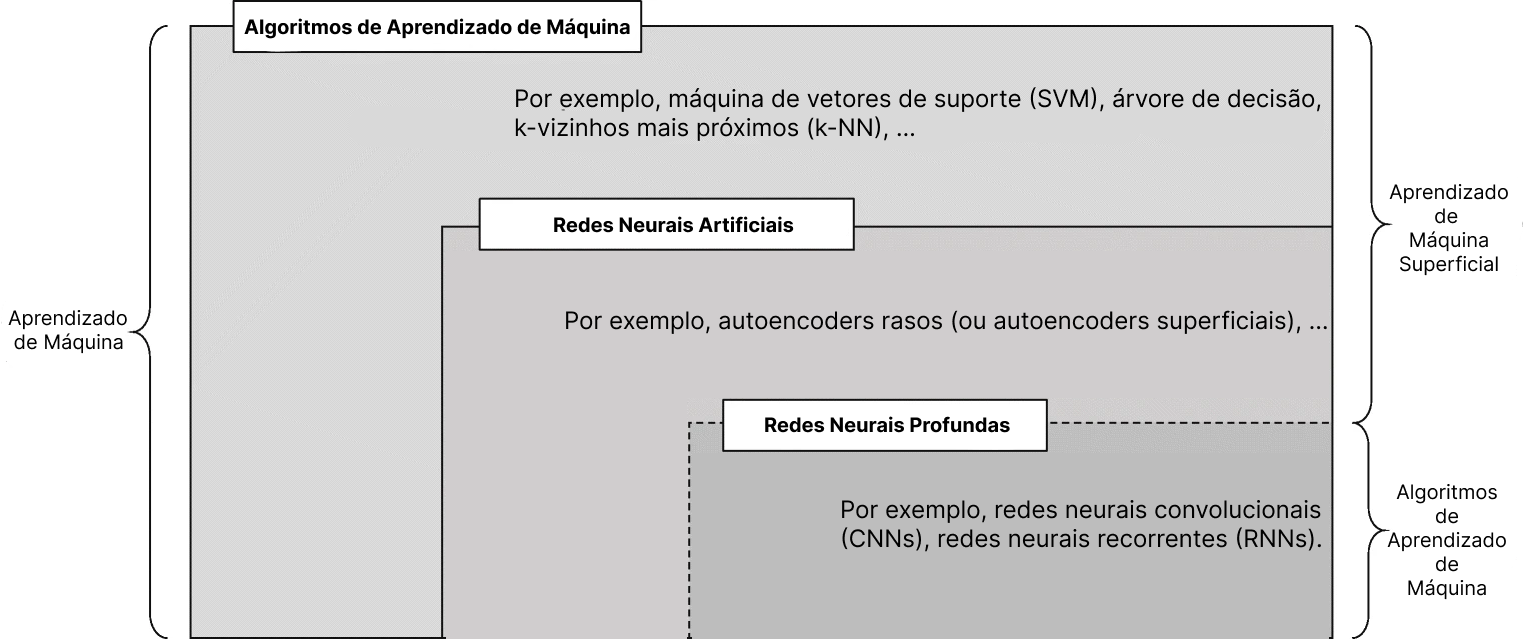
\includegraphics[width=10cm]{figures/diagrama_ann.png} % leia abaixo
	\legend{Fonte: \space\citeonline{ml_and_dp}}
	\label{fig:diagrama_ann}
\end{figure}
